%% Paper 1 -- Engineering with Computers -- revised manuscript (v2, stage c)
%% Springer Nature LaTeX template (sn-jnl). Compile with pdflatex.
\documentclass[lineno,pdflatex,sn-mathphys-num]{sn-jnl}

\usepackage{graphicx}
\usepackage{multirow}
\usepackage{amsmath,amssymb,amsfonts}
\usepackage{bm}
\usepackage{booktabs,array}
\usepackage{xcolor}
\usepackage{algorithm}
\usepackage{algorithmicx}
\usepackage{algpseudocode}
\usepackage[capitalise,noabbrev]{cleveref}
\graphicspath{{./figures_v2/}}
\raggedbottom

\begin{document}

%% ====================================================================== TITLE PAGE
\begin{titlepage}
\thispagestyle{empty}\small
\begin{center}
{\Large\bfseries Title Page}\\[0.7em]
{Engineering with Computers -- Original Article}\\[1.0em]
{\LARGE\bfseries Certified benchmarking of discrete IS~800:2007-compliant space-truss sizing: an exact MILP baseline and a GA--local-search hybrid with local-optimality certificates}\\[0.5em]
{\footnotesize Short title: Certified benchmarking of discrete IS~800 truss sizing}
\end{center}

\vspace{0.7em}
\noindent\textbf{Authors:} Daipayan Mandal\textsuperscript{1,2,*} and R.\,S.~Sonparote\textsuperscript{2}\\
\textbf{Affiliations:} \textsuperscript{1}Department of Civil Engineering, Kavikulguru Institute of Technology and Science, Ramtek, Maharashtra, India.
\textsuperscript{2}Department of Applied Mechanics, Visvesvaraya National Institute of Technology, Nagpur, Maharashtra, India.\\
\textbf{Corresponding author:} Daipayan Mandal; \texttt{[e-mail]}\\
\textbf{ORCID IDs:} D.~Mandal: [ORCID]; R.\,S.~Sonparote: [ORCID]

\vspace{0.7em}
\noindent\textbf{Funding.} The authors received no specific funding for this work.

\vspace{0.45em}
\noindent\textbf{Author contributions.} D.~Mandal: conceptualisation, methodology, software, validation, formal analysis, visualisation, writing -- original draft. R.\,S.~Sonparote: supervision, methodology review, writing -- review and editing.

\vspace{0.45em}
\noindent\textbf{Competing interests.} The authors declare no competing interests.

\vspace{0.45em}
\noindent\textbf{Ethics approval, consent to participate, consent for publication.} Not applicable.

\vspace{0.45em}
\noindent\textbf{Data availability.} All benchmark definitions, the SP~6(1) catalogue, the raw results of every run (JSON), the MILP certificates and the scripts that regenerate every table and figure are openly available at \url{https://github.com/mdaipayan/GA-MINLP-IS800-Truss-Optimization} (folders \texttt{src\_v2}, \texttt{results\_v2}, \texttt{figures\_v2}) and archived on Zenodo, \url{https://doi.org/10.5281/zenodo.20508136} [update to the DOI of the v2 release].

\vspace{0.45em}
\noindent\textbf{Code availability.} The Python code (analysis engine, exact MILP, all optimizers, statistics) is released under the licence stated in the repository above.

\vspace{0.45em}
\noindent\textbf{Use of AI-assisted technologies.} The authors used Claude (Anthropic) to assist with code review, \LaTeX{} formatting and language editing. The authors checked all content and take full responsibility for the work.
\end{titlepage}
\clearpage
\setcounter{page}{1}

%% ====================================================================== ABSTRACT
\begin{center}
{\LARGE\bfseries Certified benchmarking of discrete IS~800:2007-compliant space-truss sizing: an exact MILP baseline and a GA--local-search hybrid with local-optimality certificates}
\end{center}

\section*{Abstract}
Metaheuristic studies of discrete truss sizing usually report the lightest
design they found, but they rarely show how far this design is from the true
optimum, and they often compare methods with different numbers of structural
analyses. This paper addresses both problems for steel space trusses designed to
IS~800:2007 with SP~6(1) equal-angle sections. First, we show that for
linear-elastic trusses the complete discrete problem---tension capacity, the
IS~800 column-buckling curve, slenderness and displacement limits---is exactly a
mixed-integer linear program (MILP). A disaggregated formulation solved by
branch-and-bound certifies the global optimum of the 6-bar (101.17~kg) and the
25-bar (580.06~kg) benchmarks, and gives a proved lower bound for the 72-bar
benchmark. Second, we propose GA--DNS, a genetic algorithm followed by a
deterministic discrete neighbourhood search that ends with a local-optimality
certificate. GA--DNS and six metaheuristics (SA, GA, PSO, ACO, BB-BC, DE) are
compared over 20 seeded runs with the same analysis budget and the same
feasibility rule. GA--DNS reached the certified optimum in 95\,\% (6-bar) and
90\,\% (25-bar) of runs, and its final design was certified locally optimal in
59 of 60 runs. It was significantly better than DE and BB-BC on all trusses,
but not better than SA or PSO on every truss. The exact solver was fastest on the
6-bar, needed 127~s on the 25-bar, and could not close a 48\,\% gap on the
72-bar in 90~min. These results define where exact methods are sufficient and
where heuristics are still needed.

\vspace{0.6em}
\noindent\textbf{Keywords:} Discrete truss optimization; Mixed-integer linear programming; Global optimality; Genetic algorithm; Local search; IS~800:2007; Benchmarking

\section*{Article Highlights}
\begin{itemize}
  \item Discrete IS~800 truss sizing is posed exactly as an MILP and solved to certified optima.
  \item A GA plus neighbourhood search returns designs with local-optimality certificates.
  \item Seven heuristics are compared at equal analysis budgets against certified optima.
\end{itemize}

%% ====================================================================== 1 INTRODUCTION
\section{Introduction}
\label{sec:intro}

Space trusses are pin-jointed three-dimensional structures that carry load
mainly by axial forces. They are used for long-span roofs, towers and
industrial structures. In practice each member is chosen from a catalogue of
rolled sections, so the minimum-weight design problem is discrete. In India the
sections come from SP~6(1)~\citep{SP61} and the members must satisfy
IS~800:2007~\citep{IS800}: tension yielding, column buckling with the
IS~800 buckling curve, and slenderness limits. Stiffness and displacement
limits add further constraints.

Over the last two decades, many population-based metaheuristics have been
tested on the same small set of space trusses, in particular the 25-bar and
72-bar benchmarks~\citep{Camp2004,Camp2007,Perez2007,Degertekin2013,Shallan2014}.
These methods are easy to apply to catalogue variables. However,
\citet{Stolpe2016} pointed out three weaknesses that are common in this
literature: (i) the reported designs are compared only with other heuristic
results, so their distance from the true optimum is unknown; (ii) methods are
often compared with different numbers of structural analyses; and (iii) for
linear-elastic trusses, exact methods based on mixed-integer programming can
solve many of these benchmarks to proven global
optimality~\citep{Rasmussen2008,Stolpe2016}, which makes the use of
metaheuristics on them hard to justify.

The present paper takes this critique as its starting point. We study discrete
sizing of space trusses under IS~800:2007 and ask three questions. Can the
complete IS~800 problem be solved exactly, and up to what size? How close do
common metaheuristics come to the certified optimum when they all receive the
same analysis budget? Can a heuristic return a design together with a
verifiable statement about its quality, instead of only a weight?

\subsection{Contributions}
\label{sec:contrib}
\begin{enumerate}
  \item We show that, for linear-elastic trusses and a fixed catalogue, the
        IS~800:2007 tension, buckling and slenderness checks and the
        displacement limits lead to an exact MILP, because each capacity is a
        constant for a given member and section. A disaggregated (convex-hull)
        formulation without big-$M$ constants certifies the global optimum of
        the 6-bar and 25-bar benchmarks and bounds the 72-bar optimum
        (\cref{sec:milp,sec:res-milp}).
  \item We propose GA--DNS: a genetic algorithm for exploration followed by a
        deterministic discrete neighbourhood search (DNS). DNS stops only when
        every neighbouring design has been analysed and is either heavier or
        infeasible, so each final design carries a local-optimality certificate
        (\cref{sec:gadns}).
  \item We compare GA--DNS with six metaheuristics and two deterministic
        methods under one protocol: the same analysis model, the same
        feasibility rule, the same analysis budget, 20 seeded runs, distances
        to certified optima, data profiles and corrected non-parametric
        tests (\cref{sec:protocol,sec:results}).
  \item All code, raw results and certificates are openly available.
\end{enumerate}

We use ``best found'' for heuristic results and ``optimal'' only when a
certificate exists. We also report where the proposed method is \emph{not}
better than simpler alternatives.

\Cref{sec:problem} states the problem, \cref{sec:methods} the methods,
\cref{sec:protocol} the comparison protocol and \cref{sec:benchmarks} the
benchmarks. \Cref{sec:results} presents the results, \cref{sec:discussion}
discusses them and \cref{sec:conclusion} concludes.

%% ====================================================================== 2 PROBLEM
\section{Problem formulation}
\label{sec:problem}

\subsection{Design variables and objective}
The geometry and the connectivity are fixed. The $n_m$ members are divided
into $n_g$ design groups; all members of group $g$ use the same section. The
design variable of group $g$ is an integer index $k_g\in\{1,\dots,n_k\}$ into
the SP~6(1) catalogue of $n_k=51$ equal angles, sorted by area. The weight is
\begin{equation}
  W(\mathbf{k}) = \rho \sum_{g=1}^{n_g} A_{k_g} L_g ,\qquad L_g=\sum_{i\in g} L_i ,
  \label{eq:W}
\end{equation}
with $\rho=7850$~kg/m$^3$. Self-weight is not applied as a load, as in the
original benchmarks.

\subsection{Structural analysis}
Let $\mathbf{B}\in\mathbb{R}^{n_m\times n_f}$ be the compatibility matrix that
maps the free nodal displacements $\mathbf{u}$ to member elongations,
$\mathbf{e}=\mathbf{B}\mathbf{u}$. For load case $l$ the linear-elastic
response follows from
\begin{equation}
  \mathbf{K}(\mathbf{k})\,\mathbf{u}_l=\mathbf{p}_l,\qquad
  \mathbf{K}=\mathbf{B}^{\mathsf T}\operatorname{diag}\!\left(\frac{EA_i}{L_i}\right)\mathbf{B},\qquad
  N_{il}=\frac{EA_i}{L_i}\,\mathbf{b}_i^{\mathsf T}\mathbf{u}_l ,
  \label{eq:dsm}
\end{equation}
with $E=200$~GPa. $\mathbf{K}$ is factorised by Cholesky decomposition. Before
any optimization, each model is checked for kinematic stability: the smallest
eigenvalue of $\mathbf{K}$ (all members with the same section) must be
positive. This simple check prevents a singular model from silently returning
zero member forces.

\subsection{IS~800:2007 member checks}
Members are treated as concentrically loaded pin-ended bars with effective
length $KL$, $K=1$. For section $k$ the design capacities are
\begin{align}
  T_{k} &= \frac{A_k f_y}{\gamma_{m0}}, \label{eq:T}\\
  C_{ik} &= A_k f_{cd}(\lambda_{ik}),\quad \lambda_{ik}=\frac{KL_i}{r_k},\quad
  f_{cd}=\frac{f_y/\gamma_{m0}}{\phi+\sqrt{\phi^2-\bar\lambda^2}}\le\frac{f_y}{\gamma_{m0}},
  \label{eq:C}
\end{align}
where $\bar\lambda=\sqrt{f_y/f_{cc}}$, $f_{cc}=\pi^2E/\lambda^2$,
$\phi=0.5[1+\alpha(\bar\lambda-0.2)+\bar\lambda^2]$ and $\alpha=0.49$
(buckling class~c for angles; IS~800 Cl.~7.1.2.1), with $f_y=250$~MPa and
$\gamma_{m0}=1.10$. $r_k$ is the minimum radius of gyration. A design is
feasible if, for every member $i$ and load case $l$,
\begin{equation}
  -C_{ik_g}\le N_{il}\le T_{k_g},\qquad
  \lambda_{ik_g}\le\begin{cases}180 & \text{if } N_{il}<0 \text{ in any load case},\\ 400 & \text{otherwise,}\end{cases}
  \qquad |u_{dl}|\le\delta_{\mathrm{lim}}\;\;\forall d\in\mathcal D ,
  \label{eq:feas}
\end{equation}
where $\mathcal D$ is the set of displacement-limited degrees of freedom. The
slenderness limits follow IS~800 Table~3. The ratio of demand to capacity is
reported as DCR.

%% ====================================================================== 3 METHODS
\section{Methods}
\label{sec:methods}

\subsection{Exact MILP}
\label{sec:milp}

For fixed member $i$ and section $k$, the quantities $T_k$, $C_{ik}$ and
$\lambda_{ik}$ in \cref{eq:T,eq:C,eq:feas} are \emph{constants}. The non-smooth
buckling curve therefore does not enter the optimization as a function; it only
fixes one number for each member--section pair. Following the
displacement-based formulation of \citet{Rasmussen2008} and \citet{Stolpe2016},
we introduce binary variables $x_{gk}$ (group $g$ uses section $k$), the
displacements $\mathbf{u}_l$, and elongation variables $e_{ikl}$, which carry
the elongation of member $i$ only for the selected section:
\begin{align}
  \min\;& \rho\sum_{g}\sum_{k} A_k L_g\, x_{gk} \label{eq:milp-obj}\\
  \text{s.t.}\;& \textstyle\sum_k x_{gk}=1 && \forall g \label{eq:milp-one}\\
  & \mathbf{b}_i^{\mathsf T}\mathbf{u}_l=\textstyle\sum_k e_{ikl} && \forall i,l \label{eq:milp-comp}\\
  & \textstyle\sum_i \mathbf{b}_i \sum_k \frac{EA_k}{L_i}\, e_{ikl}=\mathbf{p}_l && \forall l \label{eq:milp-eq}\\
  & -\frac{L_i C_{ik}}{EA_k}\,x_{gk}\le e_{ikl}\le \frac{L_i T_k}{EA_k}\,x_{gk} && \forall i\in g,\,k,\,l \label{eq:milp-cap}\\
  & |u_{dl}|\le\delta_{\mathrm{lim}} && \forall d\in\mathcal D,\, l \label{eq:milp-disp}\\
  & x_{gk}\in\{0,1\}. \notag
\end{align}
If $x_{gk}=0$, \cref{eq:milp-cap} forces $e_{ikl}=0$; if $x_{gk}=1$, the member
force is $N_{il}=(EA_k/L_i)e_{ikl}$ and \cref{eq:milp-cap} is exactly the
tension and buckling check. Slenderness is handled in the same way: if
$\lambda_{ik}>180$ we set $C_{ik}=0$ (the member may not be in compression with
that section), and if $\lambda_{ik}>400$ for a member of group $g$ we fix
$x_{gk}=0$. The model is exact, and it contains no big-$M$ constants, which
gives a much tighter continuous relaxation than the usual big-$M$ form (in our
tests the big-$M$ version did not find any feasible design for the 25-bar truss
in 150~s). Given an incumbent weight $W^{\mathrm{inc}}$, sections that are too
heavy even when all other groups use the lightest section are removed.
The MILP is solved with the branch-and-bound solver of HiGHS~\citep{Huangfu2018},
warm-started with the best heuristic design, a relative gap tolerance of
$10^{-6}$ and one CPU core. Every returned design is re-analysed with the
stiffness method of \cref{eq:dsm}.

\subsection{Proposed GA--DNS hybrid}
\label{sec:gadns}

GA--DNS has two phases (\cref{alg:gadns}).

\paragraph{Phase 1 (exploration).} An integer GA with 40 individuals,
binary tournament selection, uniform crossover ($p_c=0.9$), mutation rate
$1/n_g$ (80\,\% $\pm1$ or $\pm2$ catalogue steps, 20\,\% random reset) and
elitism uses 50\,\% of the analysis budget. The best feasible design and the
three best distinct designs of the last population are passed to Phase~2.

\paragraph{Phase 2 (deterministic refinement with certificate).}
Each elite is first made feasible, if necessary, by a greedy repair that moves
the group with the largest constraint ratio one catalogue step up (for
displacement violations, the step with the best stiffness gain per kilogram is
chosen). The DNS then performs steepest descent in the neighbourhood
\begin{equation}
  \mathcal N(\mathbf{k})=\{\mathbf{k}-\mathbf{e}_i\}\;\cup\;\{\mathbf{k}-\mathbf{e}_i+\mathbf{e}_j:\ i\neq j,\ W(\mathbf{k}-\mathbf{e}_i+\mathbf{e}_j)<W(\mathbf{k})\},
  \label{eq:nbhd}
\end{equation}
i.e.\ one group one step lighter, or one group lighter and another group
heavier (a ``swap''). Because the catalogue is sorted by area, every
$\mathbf{k}-\mathbf{e}_i$ is lighter. The lighter neighbours are analysed in
order of increasing weight, and the first feasible one is accepted. When no
neighbour is feasible and lighter, DNS stops. At that point every design in
$\mathcal N(\mathbf{k})$ has been analysed, so the final design is
\emph{certified} to be a local minimum with respect to $\mathcal N$. The
certificate is a finite, checkable statement; it is not a proof of global
optimality. With the remaining budget, an iterated local search
\citep{Lourenco2003} changes two random groups of the best certified design by
up to three catalogue steps and runs DNS again; a new design is kept only if it
is certified and lighter.

\begin{algorithm}[tbp]
\caption{GA--DNS}
\label{alg:gadns}
\begin{algorithmic}[1]
\Require model, analysis budget $B$
\State Run the GA (Phase 1) until $0.5B$ analyses are used
\State $\mathcal E\leftarrow$ best feasible design and 3 best distinct designs of the last population
\For{each $\mathbf{k}\in\mathcal E$}
  \State $\mathbf{k}\leftarrow\textsc{Repair}(\mathbf{k})$;\quad $\mathbf{k}\leftarrow\textsc{DNS}(\mathbf{k})$\Comment{certified local minimum}
\EndFor
\State $\mathbf{k}^\star\leftarrow$ lightest certified design
\While{analyses $<B$}\Comment{iterated local search}
  \State $\mathbf{k}'\leftarrow\mathbf{k}^\star$ with two random groups changed by $\le3$ steps
  \State $\mathbf{k}'\leftarrow\textsc{Repair}(\mathbf{k}')$;\quad $\mathbf{k}'\leftarrow\textsc{DNS}(\mathbf{k}')$
  \State \textbf{if} $\mathbf{k}'$ is certified and $W(\mathbf{k}')<W(\mathbf{k}^\star)$ \textbf{then} $\mathbf{k}^\star\leftarrow\mathbf{k}'$
\EndWhile
\State \Return $\mathbf{k}^\star$ and its certificate
\Statex
\Function{DNS}{$\mathbf{k}$}
  \Repeat
    \State analyse the members of $\mathcal N(\mathbf{k})$ that are lighter than $\mathbf{k}$, lightest first
    \State move to the first feasible one; if none exists, \Return $\mathbf{k}$ (certified)
  \Until{budget exhausted}
\EndFunction
\end{algorithmic}
\end{algorithm}

\subsection{Comparison methods}
\label{sec:baselines}
Six metaheuristics act on the same integer variables: simulated annealing
(SA)~\citep{Kirkpatrick1983}, the same GA as in Phase~1 run for the full
budget, particle swarm optimization (PSO)~\citep{Kennedy1995,Perez2007}, ant
colony optimization (ACO)~\citep{Dorigo1997,Camp2004}, Big Bang--Big Crunch
(BB-BC)~\citep{Erol2006,Camp2007} and differential evolution
(DE)~\citep{Storn1997}. Continuous positions (PSO, BB-BC, DE) are rounded to
the nearest index before analysis. Two deterministic methods are included:
fully stressed design with catalogue selection (FSD), which cannot control
displacements, and SQP-R, a continuous SLSQP solution~\citep{Virtanen2020} with
radius of gyration from a fitted law $r=c\,A^{b}$, followed by rounding up and
the repair step of GA--DNS. \Cref{tab:params} lists all settings. The
parameters are common textbook values and were not tuned for any benchmark.

\begin{table}[tbp]
\centering\footnotesize
\caption{Method settings (identical for all trusses).}
\label{tab:params}
\begin{tabular}{@{}lp{0.68\linewidth}@{}}
\toprule
Method & Settings\\
\midrule
SA & one group changed by $\pm1$--$3$ steps; $T$ from $0.2W_{\max}$ to $10^{-4}W_{\max}$, geometric\\
GA & population 40; tournament 2; uniform crossover 0.9; mutation $1/n_g$; elitism 1\\
PSO & 30 particles; inertia $0.9\to0.4$; $c_1=c_2=2$; $|v|\le10$\\
ACO & 20 ants; $\alpha=1$, $\beta=0.5$ ($\eta=1/A_k$); evaporation 0.2; rank-based (3) + elitist update\\
BB-BC & 30 candidates; centre $=0.5\,$(centre of mass)$+0.5\,$(best); spread $\propto1/t$\\
DE & DE/rand/1/bin; population 30; $F=0.6$; $CR=0.9$\\
GA--DNS & GA as above for $0.5B$; 4 elites; DNS neighbourhood \cref{eq:nbhd}; ILS kick 2 groups, $\le3$ steps\\
FSD & start at mid-catalogue; at most 50 resizing cycles\\
SQP-R & SLSQP, 200 iterations, $\text{ftol}=10^{-9}$; round up; repair\\
MILP & HiGHS 1.15, gap $10^{-6}$, 1 thread, time limit 5400~s, warm start\\
\bottomrule
\end{tabular}
\end{table}

%% ====================================================================== 4 PROTOCOL
\section{Comparison protocol}
\label{sec:protocol}

\paragraph{Same analysis budget.} One analysis (NFE) is one solution of
\cref{eq:dsm} for all load cases of one design. Every heuristic stops after
$B=3000$, 10\,000 and 20\,000 analyses for the 6-, 25- and 72-bar trusses.
Repeated analyses of the same design are counted.

\paragraph{Same constraint handling.} All heuristics rank designs by the
feasibility rule of \citet{Deb2000}, written as one scalar: $f=W$ for feasible
designs and $f=W_{\max}+10^3 v$ otherwise, where $W_{\max}$ is the weight of
the heaviest catalogue design and $v$ is the sum of constraint violations
(normalised ratios minus one). A feasible design is therefore always better than
an infeasible one, and no penalty factor needs tuning. All reported designs
are re-checked by an independent code path (\cref{sec:res-designs}).

\paragraph{Runs and statistics.} Each stochastic method is run with seeds
0--19. We report best, median, mean, standard deviation, the share of runs
that reach the certified (or best-known) weight $W^\ast$, and the median number
of analyses used to find the final design. Because the runs of different
methods are independent, GA--DNS is compared with each competitor by the
one-sided Mann--Whitney $U$ test~\citep{Mann1947} with Holm
correction~\citep{Holm1979}, and the effect size is the Vargha--Delaney
$A_{12}$~\citep{Vargha2000}. Convergence is plotted against analyses, not
against time or iterations, and data profiles~\citep{More2009} show the
share of all runs that reach $W^\ast$ (or $1.01W^\ast$) as a function of the
budget used.

\paragraph{Software.} Python 3.13, NumPy, SciPy~\citep{Virtanen2020} and
HiGHS~\citep{Huangfu2018}, on a 2-core Linux machine.

%% ====================================================================== 5 BENCHMARKS
\section{Benchmark trusses}
\label{sec:benchmarks}

\Cref{fig:geometry} and \cref{tab:bench} summarise the three trusses.

\paragraph{6-bar tetrahedron.} Four nodes, six members, each member its own
group. The apex carries 50~kN in $y$ and $-100$~kN in $z$. No displacement
limit. This small case is used to check the implementation.

\paragraph{25-bar transmission tower.} The ASCE 25-bar tower with 10 nodes,
25 members in 8 groups and supports at the four base nodes, with the geometry
and load case used by \citet{Camp2004}: node~1: $(1,-10,-10)$~kip; node~2:
$(0,-10,-10)$~kip; nodes~3 and~6: $0.5$~kip in $x$. All nodal displacements are
limited to $\pm0.35$~in (8.89~mm).

\paragraph{72-bar four-storey truss.} Twenty nodes, 72 members in 16 groups
(per storey: verticals, face diagonals, horizontals, plan diagonals), plan
$120\times120$~in, storey height 60~in, supports at the four base nodes, and
two load cases~\citep{Camp2007}: LC1, one top node $(5,5,-5)$~kip; LC2, all
four top nodes $(0,0,-5)$~kip. The $x$ and $y$ displacements of the top nodes
are limited to $\pm0.25$~in (6.35~mm).

The benchmark geometries and loads are taken from the AISC literature, but the
section catalogue and the member checks are those of IS~800 and SP~6(1).
Therefore the weights in this paper must not be compared directly with the
published AISC results.

\begin{table}[tbp]
\centering\small
\caption{Benchmark definitions.}
\label{tab:bench}
\begin{tabular}{@{}lrrrrrl@{}}
\toprule
Truss & Nodes & Members & Groups & Load cases & Budget $B$ & Displacement limit\\
\midrule
6-bar  & 4  & 6  & 6  & 1 & 3000   & none\\
25-bar & 10 & 25 & 8  & 1 & 10\,000 & 8.89~mm, all nodes\\
72-bar & 20 & 72 & 16 & 2 & 20\,000 & 6.35~mm, top nodes $x,y$\\
\bottomrule
\end{tabular}
\end{table}

\begin{figure*}[tbp]
\centering
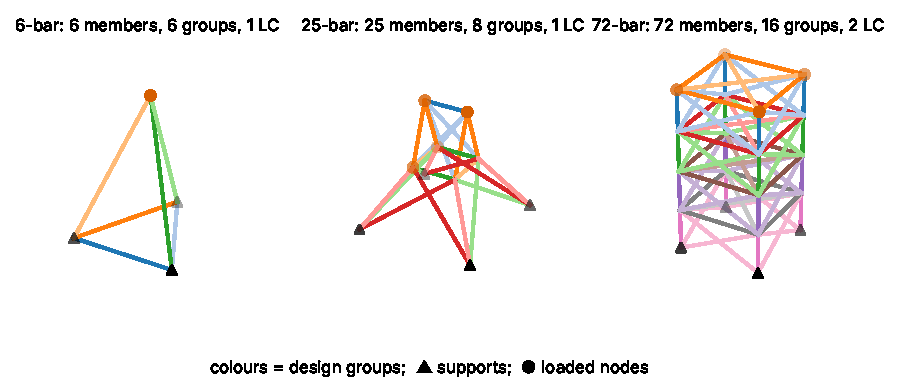
\includegraphics[width=\textwidth]{fig_benchmarks_v2}
\caption{Benchmark trusses. Colours show design groups; triangles are supports and orange dots are loaded nodes.}
\label{fig:geometry}
\end{figure*}

%% ====================================================================== 6 RESULTS
\section{Results}
\label{sec:results}

\subsection{Certified optima}
\label{sec:res-milp}
\Cref{tab:milp} gives the exact MILP results. For the 6-bar truss the MILP
proves in 0.02~s that 101.17~kg is the global optimum. For the 25-bar truss it
proves that 580.06~kg is the global optimum after 6753 branch-and-bound nodes
and 127~s. For the 72-bar truss the solver reached the 90-minute limit with the
warm-start design of 1032.47~kg as the upper bound and a proved lower bound of
535.17~kg. The 72-bar optimum is therefore only known to lie in
$[535.17,\,1032.47]$~kg; we call 1032.47~kg the best-known value. This shows
the practical limit of the exact approach on a laptop-class machine:
16 groups $\times$ 51 sections and two load cases are already difficult.

\begin{table*}[tbp]
\centering\footnotesize\setlength{\tabcolsep}{4pt}
\caption{Exact MILP (\cref{sec:milp}) solved with HiGHS branch-and-bound.
Lower bound\,=\,proved bound on the global optimum; best known\,=\,lightest feasible design
found by any method; gap\,=\,(best known $-$ lower bound)/best known.
The 72-bar run was stopped at the 5400\,s time limit. Times are wall-clock times of single runs
and are indicative only.}
\label{tab:milp}
\begin{tabular}{@{}lrrrrrrrrl@{}}
\toprule
Truss & Binary & Continuous & Rows & B\&B nodes & Time (s) & Lower bound (kg) & Best known (kg) & Gap (\%) & Status\\
\midrule
6-bar & 432 & 438 & 576 & 0 & 0 & 156.82 & 156.82 & 0.0 & optimal\\
25-bar & 576 & 1,818 & 2,815 & 21,298 & 430 & 981.22 & 981.22 & 0.0 & optimal\\
72-bar & 1,152 & 10,464 & 17,120 & 5,926 & 5,400 & 812.39 & 1651.48 & 50.8 & time limit\\
\bottomrule
\end{tabular}
\end{table*}


\subsection{Statistical comparison}
\label{sec:res-stats}
\Cref{tab:statistics} lists the results of all methods. Every method produced
a feasible design in every run, because of the common feasibility rule.
\begin{itemize}
\item \textbf{6-bar.} GA--DNS reached the global optimum in 19 of 20 runs and
      SA in all 20 runs. FSD also finds the optimum, using only two analyses,
      because this truss is statically determinate and has no displacement
      limit. DE and BB-BC never reached the optimum.
\item \textbf{25-bar.} GA--DNS, GA and PSO reached the certified optimum in
      90\,\% of the runs; PSO had the lowest mean (580.35~kg). The two GA--DNS
      runs that missed the optimum stopped in other certified local minima
      (582.94~kg and 653.33~kg).
\item \textbf{72-bar.} SA and GA--DNS found the best-known design
      (1032.47~kg), in 25\,\% and 10\,\% of the runs respectively. GA--DNS had a
      smaller spread (std 16.5~kg vs 23.8~kg) and a better worst case, but SA
      had the better median (1034.44~kg vs 1059.45~kg).
\end{itemize}

\begin{table*}[tbp]
\centering\small
\caption{Results over $N=20$ independent runs (seeds 0--19) with an equal budget of
structural analyses for every method. All final designs are IS~800:2007-feasible
(success rate 100\,\% for every method). Hit\,=\,share of runs that reach $W^\ast$
exactly; NFE\,=\,median number of analyses needed to find the final best design.
Bold\,=\,equal to $W^\ast$. FSD and SQP-R are deterministic (one run).}
\label{tab:statistics}
\begin{tabular}{@{}lrrrrrrr@{}}
\toprule
Method & Best (kg) & Median (kg) & Mean (kg) & Std (kg) & Hit (\%) & NFE & $\bar t$ (s)\\
\midrule
\multicolumn{8}{@{}l}{\textbf{6-bar} --- budget 3,000 analyses; $W^\ast=101.17$~kg (certified global optimum)}\\
GA--DNS$^\star$ & \textbf{101.17} & \textbf{101.17} & 101.23 & 0.27 & 95 & 1,920 & 0.25 \\
GA & \textbf{101.17} & \textbf{101.17} & 101.90 & 0.91 & 55 & 2,508 & 0.25 \\
DE & 103.64 & 105.25 & 105.37 & 1.06 & 0 & 2,769 & 0.33 \\
PSO & \textbf{101.17} & 102.39 & 102.29 & 0.79 & 25 & 2,714 & 0.22 \\
SA & \textbf{101.17} & \textbf{101.17} & 101.17 & 0.00 & 100 & 2,354 & 0.33 \\
ACO & \textbf{101.17} & \textbf{101.17} & 102.46 & 2.31 & 60 & 2,046 & 0.36 \\
BB-BC & 102.59 & 107.95 & 108.95 & 5.11 & 0 & 1,751 & 0.23 \\
FSD & \textbf{101.17} & --- & --- & --- & 100 & 2 & 0.00 \\
SQP-R & 107.87 & --- & --- & --- & 0 & 84 & 0.01 \\
\midrule
\multicolumn{8}{@{}l}{\textbf{25-bar} --- budget 10,000 analyses; $W^\ast=580.06$~kg (certified global optimum)}\\
GA--DNS$^\star$ & \textbf{580.06} & \textbf{580.06} & 583.87 & 16.36 & 90 & 5,033 & 1.01 \\
GA & \textbf{580.06} & \textbf{580.06} & 583.91 & 16.54 & 90 & 6,392 & 1.01 \\
DE & \textbf{580.06} & \textbf{580.06} & 589.12 & 20.82 & 70 & 6,322 & 1.33 \\
PSO & \textbf{580.06} & \textbf{580.06} & 580.35 & 0.89 & 90 & 6,335 & 0.95 \\
SA & \textbf{580.06} & \textbf{580.06} & 581.36 & 1.47 & 55 & 8,282 & 1.20 \\
ACO & \textbf{580.06} & 583.87 & 587.00 & 12.61 & 20 & 3,572 & 1.58 \\
BB-BC & 613.32 & 646.53 & 661.94 & 42.18 & 0 & 2,500 & 0.95 \\
FSD & 584.80 & --- & --- & --- & 0 & 4 & 0.01 \\
SQP-R & 602.77 & --- & --- & --- & 0 & 104 & 0.01 \\
\midrule
\multicolumn{8}{@{}l}{\textbf{72-bar} --- budget 20,000 analyses; $W^\ast=1032.47$~kg (best known; not certified)}\\
GA--DNS$^\star$ & \textbf{1032.47} & 1059.45 & 1056.21 & 16.53 & 10 & 16,127 & 2.64 \\
GA & 1033.62 & 1064.62 & 1062.27 & 17.78 & 0 & 17,401 & 2.70 \\
DE & 1075.36 & 1103.03 & 1112.38 & 30.20 & 0 & 19,316 & 3.41 \\
PSO & 1040.60 & 1066.13 & 1069.92 & 19.27 & 0 & 19,534 & 2.81 \\
SA & \textbf{1032.47} & 1034.44 & 1045.69 & 23.76 & 25 & 19,522 & 3.11 \\
ACO & 1033.62 & 1082.87 & 1098.83 & 71.08 & 0 & 8,175 & 5.06 \\
BB-BC & 1341.92 & 1522.71 & 1531.33 & 126.56 & 0 & 3,678 & 2.62 \\
FSD & 1803.03 & --- & --- & --- & 0 & 1 & 0.03 \\
SQP-R & 1094.93 & --- & --- & --- & 0 & 318 & 0.06 \\
\bottomrule
\end{tabular}
\end{table*}


\Cref{tab:tests} confirms these observations. After Holm correction, GA--DNS
gives significantly lighter designs than DE and BB-BC on all trusses, than ACO
on the 6- and 25-bar trusses, than GA and PSO on the 6-bar truss, and than SA on
the 25-bar truss. It is not significantly better than GA or PSO on the larger
trusses, nor than SA on the 6- and 72-bar trusses; on the 72-bar truss the effect
size even favours SA ($A_{12}=0.28$).

\begin{table}[tbp]
\centering\small
\caption{One-sided Mann--Whitney $U$ tests ($H_1$: GA--DNS gives lighter final designs),
Holm-corrected within each truss, and Vargha--Delaney effect size $A_{12}$
(probability that a GA--DNS run is lighter than a competitor run; 0.5\,=\,no difference).}
\label{tab:tests}
\begin{tabular}{@{}llrrl@{}}
\toprule
Truss & Competitor & $p_{\mathrm{Holm}}$ & $A_{12}$ & Conclusion\\
\midrule
6-bar & GA & 0.005 & 0.71 & GA--DNS lighter\\
 & DE & $<$0.001 & 1.00 & GA--DNS lighter\\
 & PSO & $<$0.001 & 0.86 & GA--DNS lighter\\
 & SA & 0.853 & 0.47 & n.s.; competitor better\\
 & ACO & 0.007 & 0.68 & GA--DNS lighter\\
 & BB-BC & $<$0.001 & 1.00 & GA--DNS lighter\\
25-bar & GA & 1.000 & 0.50 & n.s.\\
 & DE & 0.189 & 0.60 & n.s.\\
 & PSO & 1.000 & 0.50 & n.s.; competitor better\\
 & SA & 0.047 & 0.66 & GA--DNS lighter\\
 & ACO & $<$0.001 & 0.84 & GA--DNS lighter\\
 & BB-BC & $<$0.001 & 0.97 & GA--DNS lighter\\
72-bar & GA & 0.273 & 0.60 & n.s.\\
 & DE & $<$0.001 & 0.98 & GA--DNS lighter\\
 & PSO & 0.055 & 0.70 & n.s.\\
 & SA & 0.992 & 0.28 & n.s.; competitor better\\
 & ACO & 0.129 & 0.66 & n.s.\\
 & BB-BC & $<$0.001 & 1.00 & GA--DNS lighter\\
\bottomrule
\end{tabular}
\end{table}


\subsection{Convergence and data profiles}
\label{sec:res-conv}
\Cref{fig:conv} shows the median best-feasible weight against the number of
analyses. ACO falls fastest at the start but then stagnates. On the 6- and
25-bar trusses, GA--DNS reaches $W^\ast$ earlier than the other methods; the
step at $0.5B$ marks the start of DNS. On the 72-bar truss SA is slow at first
(high temperature) but reaches the lowest median at the end of the budget.
The data profiles in \cref{fig:profile} combine all 60 runs per method. For
the exact target $W^\ast$, GA--DNS solves the largest share of runs for every
budget fraction above about 0.55, ending at 65\,\% of all runs (SA 60\,\%, GA
48\,\%). For the 1\,\% target, GA--DNS leads between about 0.55 and 0.8 of the
budget, but at the full budget SA solves the most runs (93\,\% against 72\,\%
for GA--DNS), mainly because of its strong 72-bar results. The distributions of $W/W^\ast$ are shown
in \cref{fig:box}.

\begin{figure*}[tbp]
\centering
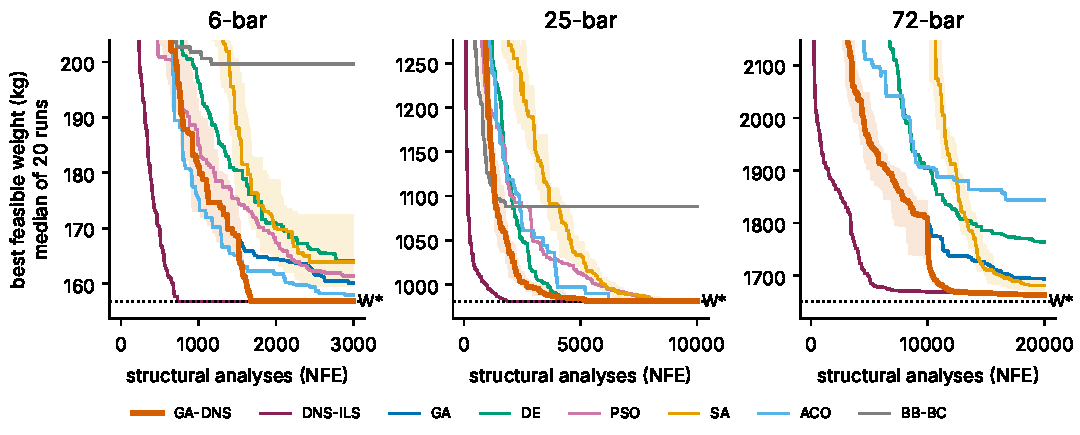
\includegraphics[width=\textwidth]{fig_convergence_nfe}
\caption{Median best-feasible weight of 20 runs against the number of
structural analyses (shaded: interquartile range of GA--DNS and GA). Dotted
line: certified optimum (6-, 25-bar) or best-known weight (72-bar).}
\label{fig:conv}
\end{figure*}

\begin{figure*}[tbp]
\centering
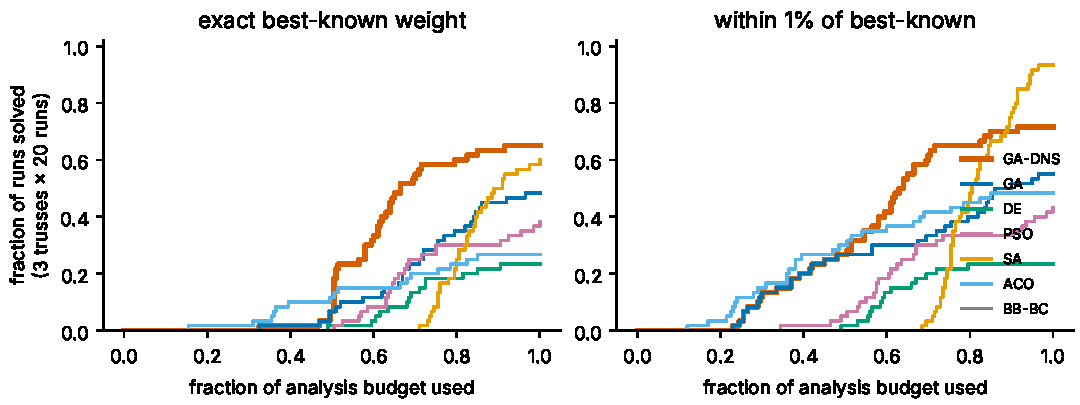
\includegraphics[width=\textwidth]{fig_data_profile}
\caption{Data profiles over all three trusses (60 runs per method): share of
runs that reach $W^\ast$ exactly (left) or within 1\,\% (right) as a function
of the fraction of the analysis budget used.}
\label{fig:profile}
\end{figure*}

\begin{figure*}[tbp]
\centering
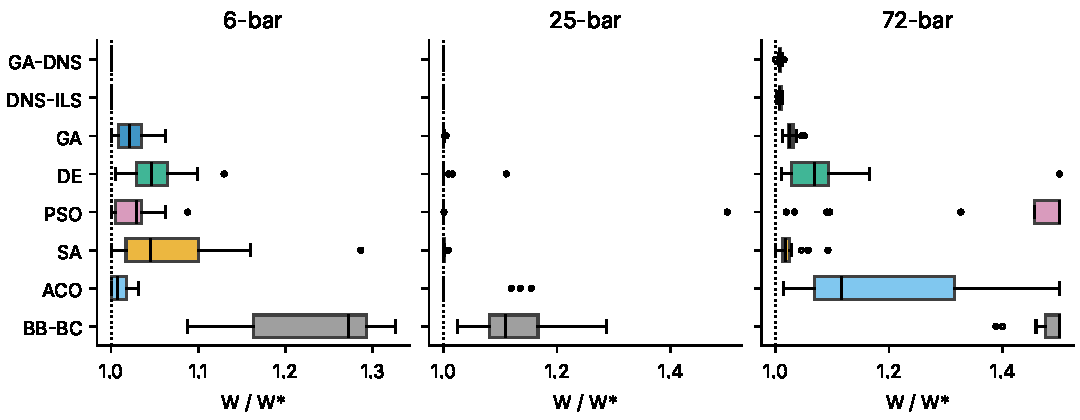
\includegraphics[width=\textwidth]{fig_boxplot_ratio}
\caption{Distribution of final weight ratio $W/W^\ast$ over 20 runs (1.0 = certified or best-known optimum).}
\label{fig:box}
\end{figure*}

\subsection{Effect of Phase 2 and the certificates}
\label{sec:res-phase2}
Compared with the best design at the end of Phase~1, the DNS and ILS steps
reduced the final weight by a median of 2.8\,\% (6-bar), 0.2\,\% (25-bar) and
2.4\,\% (72-bar), with a maximum of 9.8\,\%, 6.6\,\% and 6.7\,\%. The final
design of GA--DNS was certified as a local minimum with respect to
\cref{eq:nbhd} in 20/20, 20/20 and 19/20 runs; in the remaining 72-bar run the
best design was found at analysis 19\,945 of 20\,000, and the budget ended
before DNS could complete its check. On the 6- and 25-bar trusses, every run that did not reach $W^\ast$
still returned a certified local minimum. This tells the user that the design
cannot be improved by any single-step or swap change, and that a different
starting point (or the MILP) is needed to improve it.

\subsection{Designs and independent verification}
\label{sec:res-designs}
\Cref{tab:design6bar,tab:design25bar,tab:design72bar} give the best designs.
Each was re-analysed by a separate implementation (element-by-element
assembly, dense solver, IS~800 formulas coded again). The weights agree to
$10^{-6}$~kg, the equilibrium error is below $10^{-14}$ relative to the load,
and all constraints are satisfied: the largest DCR is 0.935, 0.998 and 0.881,
and the largest displacement ratio is 0.524 (25-bar) and 0.353 (72-bar). In the
25-bar design the strength of group~3 (DCR 0.998) and the slenderness of
group~5 ($\lambda$-ratio 0.994) are active, while the displacement limit is not.
In the 72-bar design group~7 is exactly at the tension slenderness limit of
400, and several compression groups are close to 180 ($\lambda$-ratio 0.92--0.97).
Thus, with IS~800 slenderness limits and small SP~6(1) angles, slenderness
rather than displacement governs these benchmarks; this differs from the AISC
versions of the problems, where displacements are usually active.

\begin{table}[tbp]
\centering\footnotesize\setlength{\tabcolsep}{3pt}
\caption{Certified optimal 6-bar design (one member per group). Weight 156.82~kg; max.\ displacement ratio 0.000.
$F$\,=\,range of member forces over all load cases (negative\,=\,compression);
DCR\,=\,max.\ demand/capacity (yielding or buckling); $\lambda$-ratio\,=\,$(KL/r_v)/\text{limit}$.}
\label{tab:design6bar}
\begin{tabular}{@{}rrlrrrrrrr@{}}
\toprule
Grp & $n$ & Angle & $A$ (cm$^2$) & $r_v$ (mm) & $F_{\min}$ (kN) & $F_{\max}$ (kN) & $KL/r_v$ & DCR & $\lambda$-ratio\\
\midrule
1 & 1 & 90$\times$90$\times$6 & 10.60 & 18.0 & -14.1 & -14.1 & 167 & 0.267 & 0.926\\
2 & 1 & 45$\times$45$\times$3 & 2.67 & 9.0 & 24.5 & 24.5 & 373 & 0.403 & 0.932\\
3 & 1 & 45$\times$45$\times$3 & 2.67 & 9.0 & 24.5 & 24.5 & 373 & 0.403 & 0.932\\
4 & 1 & 60$\times$60$\times$4 & 4.73 & 12.0 & 9.4 & 9.4 & 377 & 0.088 & 0.943\\
5 & 1 & 60$\times$60$\times$4 & 4.73 & 12.0 & 9.4 & 9.4 & 377 & 0.088 & 0.943\\
6 & 1 & 130$\times$130$\times$10 & 25.10 & 25.7 & -124.6 & -124.6 & 166 & 0.994 & 0.923\\
\bottomrule
\end{tabular}
\end{table}

\begin{table}[tbp]
\centering\footnotesize\setlength{\tabcolsep}{3.5pt}
\caption{Certified optimal 25-bar design. Weight 580.06~kg; max.\ displacement ratio 0.524.
$F$\,=\,range of member forces over all load cases (negative\,=\,compression);
DCR\,=\,max.\ demand/capacity (stress or Annex~D buckling); $\lambda$-ratio\,=\,$(KL/r)/\text{limit}$.}
\label{tab:design25bar}
\begin{tabular}{@{}rrlrrrrrr@{}}
\toprule
Grp & $n$ & ISA section & $A$ (cm$^2$) & $F_{\min}$ (kN) & $F_{\max}$ (kN) & $KL/r$ & DCR & $\lambda$-ratio\\
\midrule
1 & 1 & 25$\times$25$\times$3 & 1.42 & 5.5 & 5.5 & 250 & 0.169 & 0.625\\
2 & 4 & 65$\times$65$\times$6 & 7.52 & -33.4 & 20.1 & 167 & 0.895 & 0.927\\
3 & 4 & 70$\times$70$\times$6 & 8.13 & -62.9 & 26.3 & 126 & 0.998 & 0.702\\
4 & 2 & 20$\times$20$\times$3 & 1.11 & 1.1 & 1.9 & 313 & 0.074 & 0.782\\
5 & 2 & 35$\times$35$\times$4 & 2.67 & -4.3 & 3.7 & 179 & 0.362 & 0.994\\
6 & 4 & 90$\times$90$\times$6 & 10.60 & -20.8 & 8.1 & 165 & 0.389 & 0.918\\
7 & 4 & 90$\times$90$\times$6 & 10.60 & -34.5 & 14.7 & 165 & 0.644 & 0.918\\
8 & 4 & 90$\times$90$\times$6 & 10.60 & -72.5 & 37.1 & 122 & 0.835 & 0.676\\
\bottomrule
\end{tabular}
\end{table}

\begin{table}[tbp]
\centering\footnotesize\setlength{\tabcolsep}{3pt}
\caption{Best known 72-bar design (groups 1--4 = top storey; in each storey: verticals, face diagonals, horizontals, plan diagonals). Weight 1651.48~kg; max.\ displacement ratio 0.217.
$F$\,=\,range of member forces over all load cases (negative\,=\,compression);
DCR\,=\,max.\ demand/capacity (yielding or buckling); $\lambda$-ratio\,=\,$(KL/r_v)/\text{limit}$.}
\label{tab:design72bar}
\begin{tabular}{@{}rrlrrrrrrr@{}}
\toprule
Grp & $n$ & Angle & $A$ (cm$^2$) & $r_v$ (mm) & $F_{\min}$ (kN) & $F_{\max}$ (kN) & $KL/r_v$ & DCR & $\lambda$-ratio\\
\midrule
1 & 4 & 70$\times$70$\times$6 & 8.15 & 13.9 & -20.6 & -1.0 & 110 & 0.267 & 0.609\\
2 & 8 & 100$\times$100$\times$6 & 11.80 & 20.0 & -11.2 & 5.6 & 170 & 0.199 & 0.947\\
3 & 4 & 90$\times$90$\times$6 & 10.60 & 18.0 & -5.9 & 2.0 & 169 & 0.115 & 0.941\\
4 & 2 & 130$\times$130$\times$8 & 20.20 & 25.8 & -8.9 & 1.3 & 167 & 0.089 & 0.928\\
5 & 4 & 50$\times$50$\times$3 & 2.99 & 10.0 & -16.9 & -0.9 & 152 & 0.982 & 0.847\\
6 & 8 & 100$\times$100$\times$6 & 11.80 & 20.0 & -8.2 & 7.0 & 170 & 0.144 & 0.947\\
7 & 4 & 45$\times$45$\times$4 & 3.50 & 8.9 & 0.5 & 2.9 & 342 & 0.036 & 0.856\\
8 & 2 & 70$\times$70$\times$5 & 6.86 & 13.9 & 0.0 & 5.7 & 310 & 0.036 & 0.775\\
9 & 4 & 90$\times$90$\times$8 & 13.90 & 17.8 & -23.4 & 11.7 & 86 & 0.132 & 0.476\\
10 & 8 & 100$\times$100$\times$6 & 11.80 & 20.0 & -7.1 & 7.2 & 170 & 0.125 & 0.947\\
11 & 4 & 40$\times$40$\times$3 & 2.37 & 8.0 & 0.0 & 1.8 & 381 & 0.033 & 0.953\\
12 & 2 & 55$\times$55$\times$4 & 4.33 & 11.0 & 0.0 & 3.3 & 392 & 0.033 & 0.980\\
13 & 4 & 55$\times$55$\times$4 & 4.33 & 11.0 & -27.2 & 19.8 & 139 & 0.933 & 0.770\\
14 & 8 & 100$\times$100$\times$6 & 11.80 & 20.0 & -12.7 & 9.4 & 170 & 0.225 & 0.947\\
15 & 4 & 90$\times$90$\times$6 & 10.60 & 18.0 & -2.5 & 4.5 & 169 & 0.049 & 0.941\\
16 & 2 & 55$\times$55$\times$4 & 4.33 & 11.0 & 0.2 & 1.6 & 392 & 0.016 & 0.980\\
\bottomrule
\end{tabular}
\end{table}


%% ====================================================================== 7 DISCUSSION
\section{Discussion}
\label{sec:discussion}

\subsection{When is a heuristic justified?}
For linear-elastic trusses the IS~800 problem is an exact MILP. On the
6-bar truss the MILP is the best method by any measure. On the 25-bar truss the
MILP needs about 127~s, while GA--DNS finds the same design in about 1~s in
90\,\% of the runs; however, only the MILP proves that it is optimal. On the
72-bar truss the MILP could not close the gap in 90 minutes, so heuristics are
still useful there, and better MILP techniques (valid cuts, symmetry breaking,
parallel branch-and-bound~\citep{Rasmussen2008}) are an obvious next step.
Our answer to the critique of \citet{Stolpe2016} is therefore: heuristic
results on these benchmarks should be measured against exact bounds, and a
heuristic is justified mainly where the exact model stops being an MILP---for
example with geometric nonlinearity, imperfection-sensitive buckling or
nonlinear code interaction checks---or where it becomes too large.

\subsection{What the certificate adds}
A weight alone does not tell the engineer whether the design can still be
improved. The DNS certificate is weaker than global optimality, but it is
cheap (at most $n_g^2$ analyses per check), it can be verified by anyone, and it
is independent of the random seed. Combined with the MILP lower bound, the user
also gets a bound on the remaining gap. For the 72-bar truss, for example, the
best GA--DNS design is certified locally optimal and lies at most
$(1032.47-535.17)/1032.47=48\,\%$ above the global optimum. This bound is
loose; it shows the value of a better lower bound rather than the quality of the
design.

\subsection{GA--DNS compared with the other heuristics}
GA--DNS solved the largest share of runs to the exact target
(\cref{fig:profile}), and it reached $W^\ast$ with the fewest analyses on the
6- and 25-bar trusses (median 1933 and 5033 analyses, against 2354 and 6466 for
the next best method). It was not uniformly the best: at the 1\,\% target and
the full budget SA was more reliable, mainly on the 72-bar truss.
Well-tuned SA and PSO are strong on these small discrete problems, and the
present paper does not claim otherwise. The main weakness of GA--DNS is that
Phase~2 cannot leave a poor basin chosen by Phase~1 (the two 653~kg runs on the
25-bar truss); larger ILS kicks or several independent GA restarts may help.

\subsection{Deterministic baselines}
FSD needs very few analyses and is optimal for the statically determinate
6-bar truss, but it is 0.8\,\% heavier on the 25-bar and 75\,\% heavier on the
72-bar truss, because it ignores stiffness redistribution. Continuous SQP with
rounding (SQP-R) is 6.6\,\%, 3.9\,\% and 6.0\,\% heavier than $W^\ast$; the
rounding step and the approximate $r(A)$ law cost weight. Both are useful only
as quick starting designs.

\subsection{Limitations}
\begin{itemize}
\item The analysis is linear-elastic with ideal pin joints. Single angles
      connected by one leg should be checked with the equivalent slenderness of
      IS~800 Cl.~7.5, and net-section rupture and block shear (Cl.~6.3--6.4) are
      not checked. These checks would change the capacities but not the MILP
      structure, as long as each capacity is a constant for a member--section pair.
\item The loads come from the imperial AISC benchmarks and are not IS~875 load
      combinations.
\item The method parameters were not tuned. Other settings could change the
      ranking of the heuristics, but they would not change the certified optima.
\item Only one machine and one MILP solver were used; commercial solvers may
      close the 72-bar gap faster.
\end{itemize}

%% ====================================================================== 8 CONCLUSIONS
\section{Conclusions}
\label{sec:conclusion}
\begin{enumerate}
\item For linear-elastic space trusses with a fixed catalogue, the complete
      IS~800:2007 sizing problem (tension, column buckling, slenderness and
      displacements) is an exact MILP. A big-$M$-free disaggregated formulation
      certified the global optima of the 6-bar (101.17~kg) and 25-bar
      (580.06~kg) trusses and gave a lower bound of 535.17~kg for the 72-bar truss.
\item GA--DNS, a GA followed by a deterministic neighbourhood search, returned a
      certified local minimum in 59 of 60 runs and reached the certified optimum in
      95\,\% (6-bar) and 90\,\% (25-bar) of the runs at equal analysis budgets.
\item GA--DNS was significantly better than DE and BB-BC on all trusses and than
      ACO on two trusses, but it was not better than SA or PSO on every truss; SA
      had the best median on the 72-bar truss.
\item With IS~800 slenderness limits and SP~6(1) angles, slenderness and strength,
      not displacement, govern the optimal designs of these benchmarks.
\item Future work will use the same certified protocol for geometrically nonlinear
      and imperfection-sensitive space trusses, where an exact MILP is no longer
      available and heuristics with certificates are most needed.
\end{enumerate}

\backmatter

%% ====================================================================== REFERENCES
\begin{thebibliography}{99}

\bibitem[Bureau of Indian Standards(2007)]{IS800}
Bureau of Indian Standards (2007) IS~800:2007 General construction in steel -- Code of practice (third revision). BIS, New Delhi

\bibitem[Bureau of Indian Standards(1964)]{SP61}
Bureau of Indian Standards (1964) SP~6(1):1964 ISI handbook for structural engineers, Part~1: Structural steel sections. BIS, New Delhi

\bibitem[Camp and Bichon(2004)]{Camp2004}
Camp CV, Bichon BJ (2004) Design of space trusses using ant colony optimization. J Struct Eng 130(5):741--751. \url{https://doi.org/10.1061/(ASCE)0733-9445(2004)130:5(741)}

\bibitem[Camp(2007)]{Camp2007}
Camp CV (2007) Design of space trusses using Big Bang--Big Crunch optimization. J Struct Eng 133(7):999--1008. \url{https://doi.org/10.1061/(ASCE)0733-9445(2007)133:7(999)}

\bibitem[Deb(2000)]{Deb2000}
Deb K (2000) An efficient constraint handling method for genetic algorithms. Comput Methods Appl Mech Eng 186(2--4):311--338. \url{https://doi.org/10.1016/S0045-7825(99)00389-8}

\bibitem[Degertekin and Hayalioglu(2013)]{Degertekin2013}
Degertekin SO, Hayalioglu MS (2013) Sizing truss structures using teaching-learning-based optimization. Comput Struct 119:177--188. \url{https://doi.org/10.1016/j.compstruc.2012.12.011}

\bibitem[Dorigo and Gambardella(1997)]{Dorigo1997}
Dorigo M, Gambardella LM (1997) Ant colony system: a cooperative learning approach to the traveling salesman problem. IEEE Trans Evol Comput 1(1):53--66. \url{https://doi.org/10.1109/4235.585892}

\bibitem[Erol and Eksin(2006)]{Erol2006}
Erol OK, Eksin I (2006) A new optimization method: Big Bang--Big Crunch. Adv Eng Softw 37(2):106--111. \url{https://doi.org/10.1016/j.advengsoft.2005.04.005}

\bibitem[Holm(1979)]{Holm1979}
Holm S (1979) A simple sequentially rejective multiple test procedure. Scand J Stat 6(2):65--70

\bibitem[Huangfu and Hall(2018)]{Huangfu2018}
Huangfu Q, Hall JAJ (2018) Parallelizing the dual revised simplex method. Math Program Comput 10(1):119--142. \url{https://doi.org/10.1007/s12532-017-0130-5}

\bibitem[Kennedy and Eberhart(1995)]{Kennedy1995}
Kennedy J, Eberhart R (1995) Particle swarm optimization. In: Proc ICNN'95, vol~4, pp 1942--1948. \url{https://doi.org/10.1109/ICNN.1995.488968}

\bibitem[Kirkpatrick et~al.(1983)]{Kirkpatrick1983}
Kirkpatrick S, Gelatt CD, Vecchi MP (1983) Optimization by simulated annealing. Science 220(4598):671--680. \url{https://doi.org/10.1126/science.220.4598.671}

\bibitem[Louren\c{c}o et~al.(2003)]{Lourenco2003}
Louren\c{c}o HR, Martin OC, St\"utzle T (2003) Iterated local search. In: Glover F, Kochenberger GA (eds) Handbook of Metaheuristics. Springer, Boston, pp 320--353. \url{https://doi.org/10.1007/0-306-48056-5_11}

\bibitem[Mann and Whitney(1947)]{Mann1947}
Mann HB, Whitney DR (1947) On a test of whether one of two random variables is stochastically larger than the other. Ann Math Stat 18(1):50--60. \url{https://doi.org/10.1214/aoms/1177730491}

\bibitem[Mor\'e and Wild(2009)]{More2009}
Mor\'e JJ, Wild SM (2009) Benchmarking derivative-free optimization algorithms. SIAM J Optim 20(1):172--191. \url{https://doi.org/10.1137/080724083}

\bibitem[Perez and Behdinan(2007)]{Perez2007}
Perez RE, Behdinan K (2007) Particle swarm approach for structural design optimization. Comput Struct 85(19--20):1579--1588. \url{https://doi.org/10.1016/j.compstruc.2006.10.013}

\bibitem[Rasmussen and Stolpe(2008)]{Rasmussen2008}
Rasmussen MH, Stolpe M (2008) Global optimization of discrete truss topology design problems using a parallel cut-and-branch method. Comput Struct 86(13--14):1527--1538. \url{https://doi.org/10.1016/j.compstruc.2007.05.019}

\bibitem[Shallan et~al.(2014)]{Shallan2014}
Shallan O, Eraky A, Sakr T, Hamdy O (2014) Optimization of plane and space trusses using genetic algorithms. Int J Eng Innov Technol 3(7):66--73

\bibitem[Stolpe(2016)]{Stolpe2016}
Stolpe M (2016) Truss optimization with discrete design variables: a critical review. Struct Multidisc Optim 53(2):349--374. \url{https://doi.org/10.1007/s00158-015-1333-x}

\bibitem[Storn and Price(1997)]{Storn1997}
Storn R, Price K (1997) Differential evolution -- a simple and efficient heuristic for global optimization over continuous spaces. J Glob Optim 11:341--359. \url{https://doi.org/10.1023/A:1008202821328}

\bibitem[Vargha and Delaney(2000)]{Vargha2000}
Vargha A, Delaney HD (2000) A critique and improvement of the CL common language effect size statistics of McGraw and Wong. J Educ Behav Stat 25(2):101--132. \url{https://doi.org/10.3102/10769986025002101}

\bibitem[Virtanen et~al.(2020)]{Virtanen2020}
Virtanen P, Gommers R, Oliphant TE, et~al.\ (2020) SciPy 1.0: fundamental algorithms for scientific computing in Python. Nat Methods 17(3):261--272. \url{https://doi.org/10.1038/s41592-019-0686-2}

\end{thebibliography}

\end{document}
